\section{Métriques}
\label{section:codeMetrics}

Cette section traduit notre implication sur ce projet. 
Pour ce faire, nous avons repris des statistiques des répertoires GitHub du \gls{frontend} et de l'\gls{api}. 

\subsection{Statistiques}

\begin{itemize}[nosep,noitemsep,topsep=0pt,partopsep=0pt,after=\vspace*{2pt}]
    \item Nombre de lignes de code (\gls{frontend} + \gls{backend}) : 21685 + 10158 = 31843
    \begin{itemize}[nosep,noitemsep,topsep=0pt,partopsep=0pt,after=\vspace*{2pt}]
        \item Le nombre de lignes de code a été calculé en retirant tous les fichiers générés automatiquement (ex : npm install qui va créer un fichier \textit{package-lock.json}).
    \end{itemize}
    \item Nombre de pull requests résolues (\gls{frontend} + \gls{backend}) : 49 + 79 = 128
    \begin{itemize}[nosep,noitemsep,topsep=0pt,partopsep=0pt,after=\vspace*{2pt}]
        \item Nous avons beaucoup utilisé les pull requests pour garder une trace des mises à jour importantes effectuées. Cela a été extrêmement utile avec l'intégration continue en \textit{Docker} pour tester rapidement l'application avec l'une d'elles (cf. section \ref{section:docker}).
    \end{itemize}
    \item Nombre de tests fonctionnels (\gls{backend}) : 48
    \begin{itemize}[nosep,noitemsep,topsep=0pt,partopsep=0pt,after=\vspace*{2pt}]
        \item Plutôt que de tester individuellement chaque partie de l'application (comme le feraient des tests 
        unitaires\footnote{
            \href{https://fr.wikipedia.org/wiki/Test\_unitaire}{https://fr.wikipedia.org/wiki/Test\_unitaire}
        }), nous avons choisi cette approche, de type boîte noire (c.-à-d. sans connaitre le code source), qui consiste à vérifier si les spécifications (cf. section \ref{section:analyseFonctionnelle}) sont respectées par le logiciel ainsi développé.
        Cette vérification est notamment très utile en \gls{ci_cd} (cf. figure \ref{fig:GithubActionsExample}).
    \end{itemize}
    \item Couverture du code (\gls{backend}) :  100\%
    \begin{itemize}[nosep,noitemsep,topsep=0pt,partopsep=0pt,after=\vspace*{2pt}]
        \item Il s'agit de mesurer la proportion du code source exécutée lors de tests\footnote{
            Vous pouvez consulter les résultats depuis \href{https://codecov.io/gh/SourceCodeOER/sourcecode\_api/branch/master}{https://codecov.io/gh/SourceCodeOER/sourcecode\_api/branch/master}
        } : nous considérons ici la définition générale, car celle-ci peut se décliner sous d'autres formes\footnote{
            \href{https://fr.wikipedia.org/wiki/Couverture\_de\_code}{https://fr.wikipedia.org/wiki/Couverture\_de\_code}, \cite{concept_cfg},...
        }.
        Veuillez noter que nous avons exclu du calcul quelques lignes difficiles, voire impossibles à tester afin d'avoir un taux plus réaliste.
    \end{itemize}
    \item Note Codacy de qualité du code (\gls{backend} / \gls{frontend}) :  A / B
    \begin{itemize}[nosep,noitemsep,topsep=0pt,partopsep=0pt,after=\vspace*{2pt}]
        \item Il s'agit d'une plateforme qui analyse le code source pour produire diverses mesures (pourcentage de code dupliqué, complexité du code,...).
        Elle vérifie / analyse également la lisibilité du code en fonction de conventions de codage courantes\footnote{
            Vous pouvez consulter ces rapports sur \href{https://app.codacy.com/gh/SourceCodeOER/sourcecode\_api/dashboard}{https://app.codacy.com/gh/SourceCodeOER/sourcecode\_api/dashboard} et
            \href{https://app.codacy.com/gh/SourceCodeOER/sourcecode-front/dashboard}{https://app.codacy.com/gh/SourceCodeOER/sourcecode-front/dashboard}
        }.
    \end{itemize}       
\end{itemize}

\subsection{Graphe d'activité}

\texttt{SourceCode} a connu un développement plus ou moins constant durant l'année académique 2019-2020. Étant donné que le \gls{frontend} et le \gls{backend} sont intimement liés, vous pourrez constater sur le graphe \ref{figure:frontendActivity} et \ref{figure:backendActivity} que la forte activité de l'un compense l'activité au ralenti de l'autre répertoire.

\begin{figure}[H]
    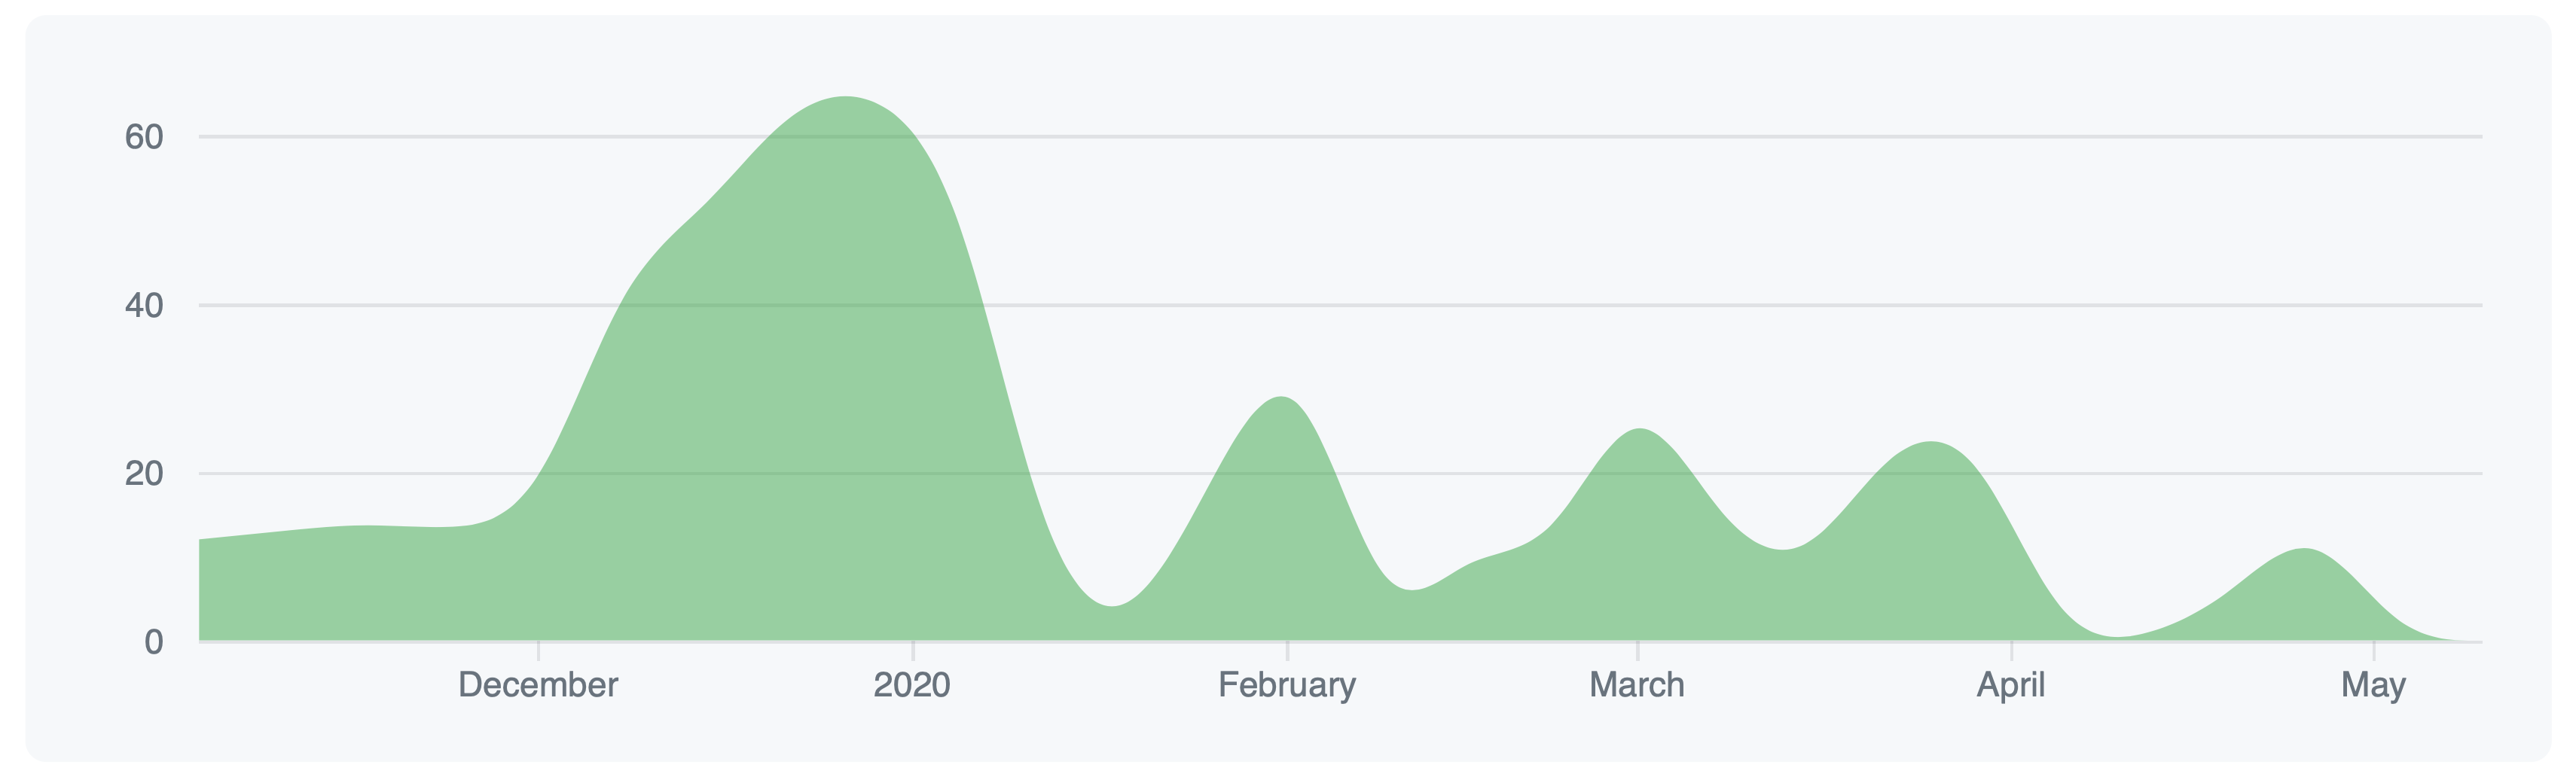
\includegraphics[width=\textwidth,height=0.3\textheight,keepaspectratio]{images/analyseCritique/graph_frontend.png}
    \centering
    \caption{GitHub : graphe d'activité (frontend)}
    \label{figure:frontendActivity}
\end{figure}

Les fonctionnalités les plus importantes comme la recherche dans la bibliothèque, la consultation d'une \gls{fiche} et la gestion des \glspl{resinfo} ont été intégrées durant la période d'octobre à janvier, après quoi nous avons amélioré l'expérience d'utilisation de l'application en appliquant quelques mises à jour et corrections de bugs jusqu'au mois de mai.\\

\begin{figure}[H]
    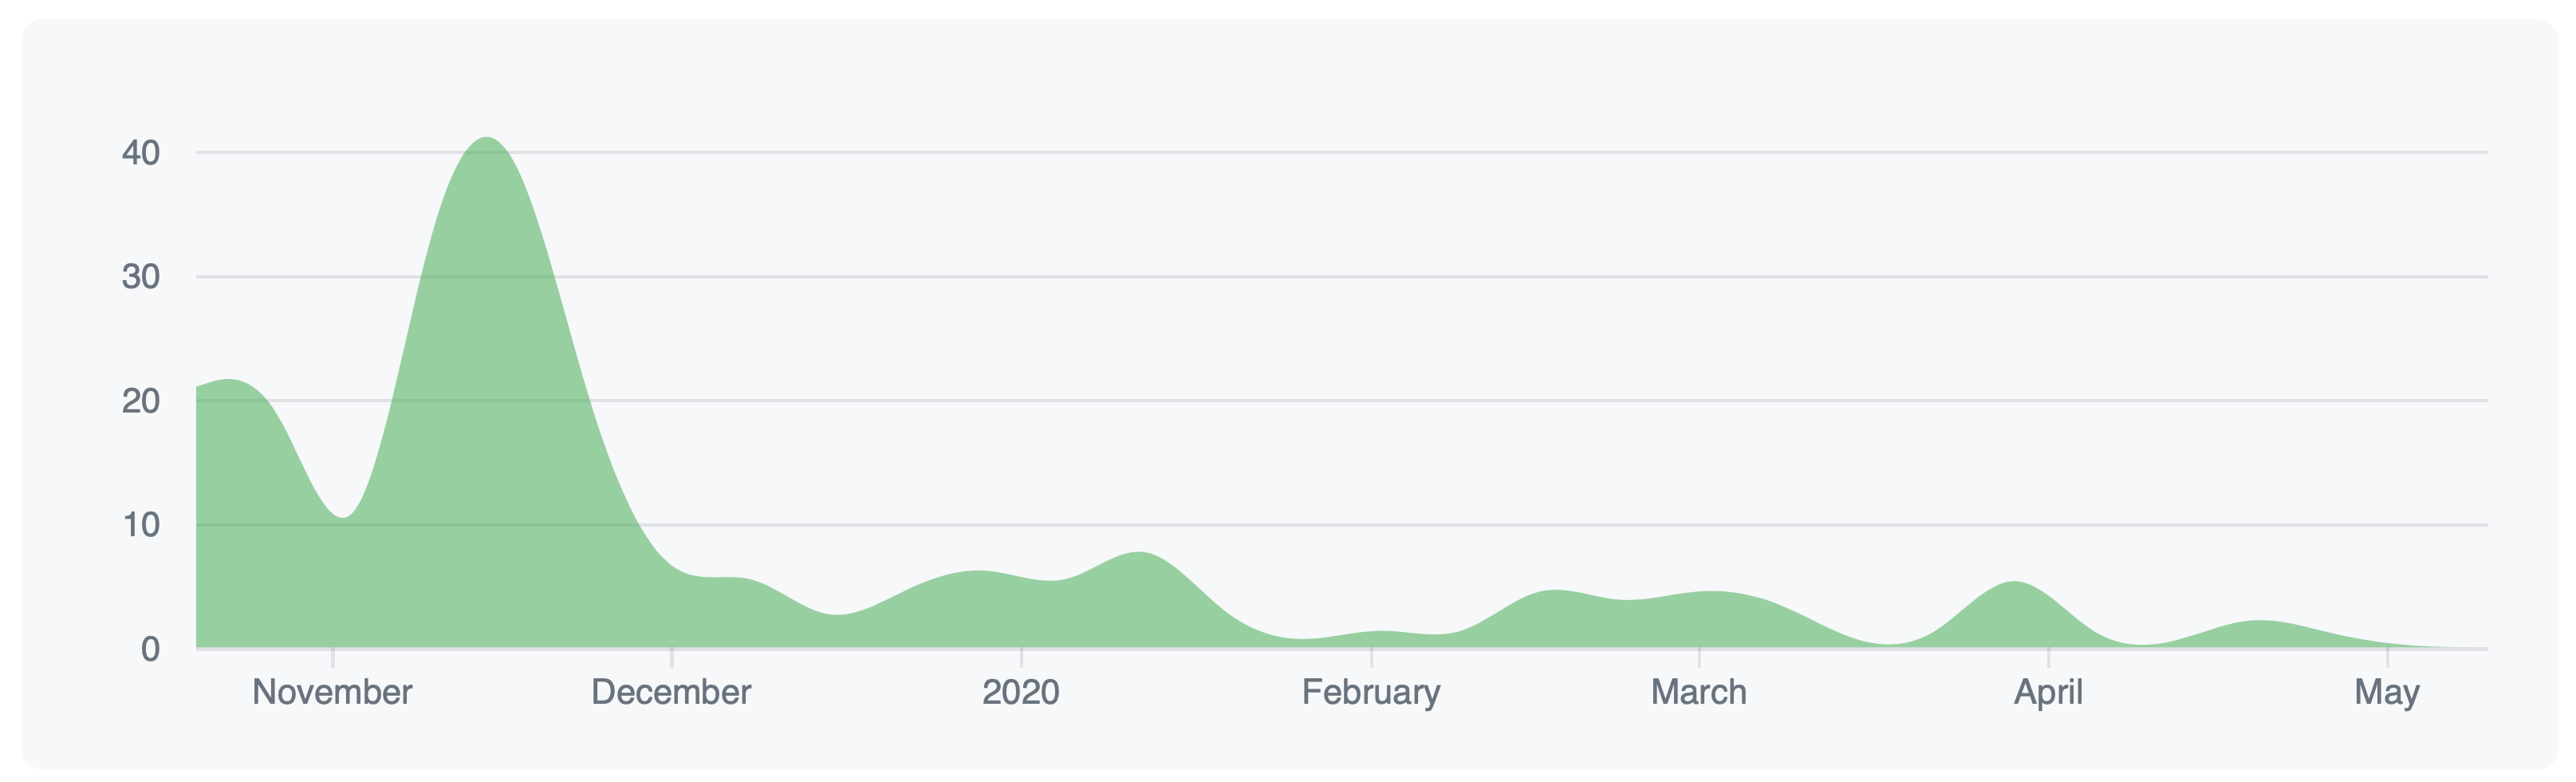
\includegraphics[width=\textwidth,height=0.3\textheight,keepaspectratio]{images/analyseCritique/graph_backend.png}
    \centering
    \caption{GitHub : graphe d'activité (backend)}
    \label{figure:backendActivity}
\end{figure}


Globalement, nous avons respecté le planning \ref{pic:ganttChart} que nous nous sommes imposé. Nous avons cependant effectué une dernière mise à jour prenant en compte un maximum des remarques relatées en section \ref{section:validationExterne}, car nous voulions prouver que \texttt{SourceCode} est capable de s'adapter aux besoins des utilisateurs.
